\documentclass[unknownkeysallowed,xcolor=table]{beamer}
 
\usepackage[T2A,T1]{fontenc}
\usepackage[utf8]{inputenc}
\usepackage[english,russian]{babel}
\usepackage{amsmath}
\usepackage{listings}
\usepackage{url}
\usepackage{textcomp}
\usepackage{multirow}
\usepackage{tikz}

\setbeamertemplate{navigation symbols}{}

\newcolumntype{C}[1]{>{\centering\let\newline\\\arraybackslash\hspace{0pt}}m{#1}}
\newcolumntype{S}[1]{>{\columncolor[HTML]{AAACED}\centering\let\newline\\\arraybackslash\hspace{0pt}}m{#1}}

\newcommand{\textapprox}{\raisebox{0.5ex}{\texttildelow}}

\newcommand{\rarr}{$\rightarrow$}
 
\colorlet{mygreen}{green!60!blue}
\colorlet{mymauve}{red!60!blue}
\definecolor{light-gray}{gray}{0.9}

\lstset{
      basicstyle=\ttfamily\small,
      commentstyle=\color{mygreen},
      keywordstyle=\color{blue},
      numberstyle=\tiny\color{blue},
      stringstyle=\color{mymauve},
      numbers=left,
      stepnumber=1,
      columns=fullflexible,
      breaklines=true,
      postbreak=\mbox{\textcolor{red}{\ensuremath{\hookrightarrow}\space}},
      literate={~} {\textapprox}{1},
      language={[11]C++}
}

\lstnewenvironment{cmdline}
  {\lstset{
      basicstyle=\ttfamily\scriptsize,
      keywordstyle=\color{blue},
      backgroundcolor=\color{light-gray},
      language={bash}
  }}
  {}

\lstnewenvironment{cmdlinelarge}
  {\lstset{
      basicstyle=\ttfamily\small,
      keywordstyle=\color{blue},
      backgroundcolor=\color{light-gray},
      language={bash}
  }}
  {}

\makeatletter
\newcommand{\srcmediumsize}{\@setfontsize{\srcmediumsize}{7pt}{7pt}}
\makeatother

\makeatletter
\newcommand{\srcbigsize}{\@setfontsize{\srcbigsize}{8pt}{8pt}}
\makeatother

\makeatletter
\newcommand{\srcsize}{\@setfontsize{\srcsize}{6pt}{6pt}}
\makeatother

\makeatletter
\newcommand{\srcsmallsize}{\@setfontsize{\srcsmallsize}{5pt}{5pt}}
\makeatother

\title[C++]
{Программирование на языке C++}
 
\subtitle{Вводный курс}
 
\author[А.~Б.~Морозов]
{
  \texorpdfstring{Александр Морозов\newline\href{mailto:gelu.speculum@gmail.com}{gelu.speculum@gmail.com}}
  {Александр Морозов}
}
  
\date[ITMO 2020]
{ИТМО, весенний семестр 2020}
 
\logo{%
  \makebox[0.97\paperwidth]{%
    
\includegraphics[align=c,width=2cm,keepaspectratio]{itmo_logo.png}
    \hfill
    
\includegraphics[align=c,width=1.5cm,keepaspectratio]{itiviti_logo.png}
  }
}

\AtBeginSection[]
{
  \begin{frame}
    \frametitle{Содержание}
    \tableofcontents[currentsection]
  \end{frame}
}

\begin{document}
 
\frame{\titlepage}

%-------------------------------------------------
\section{Текст программы и этапы его обработки}

\begin{frame}{Текст программы}
  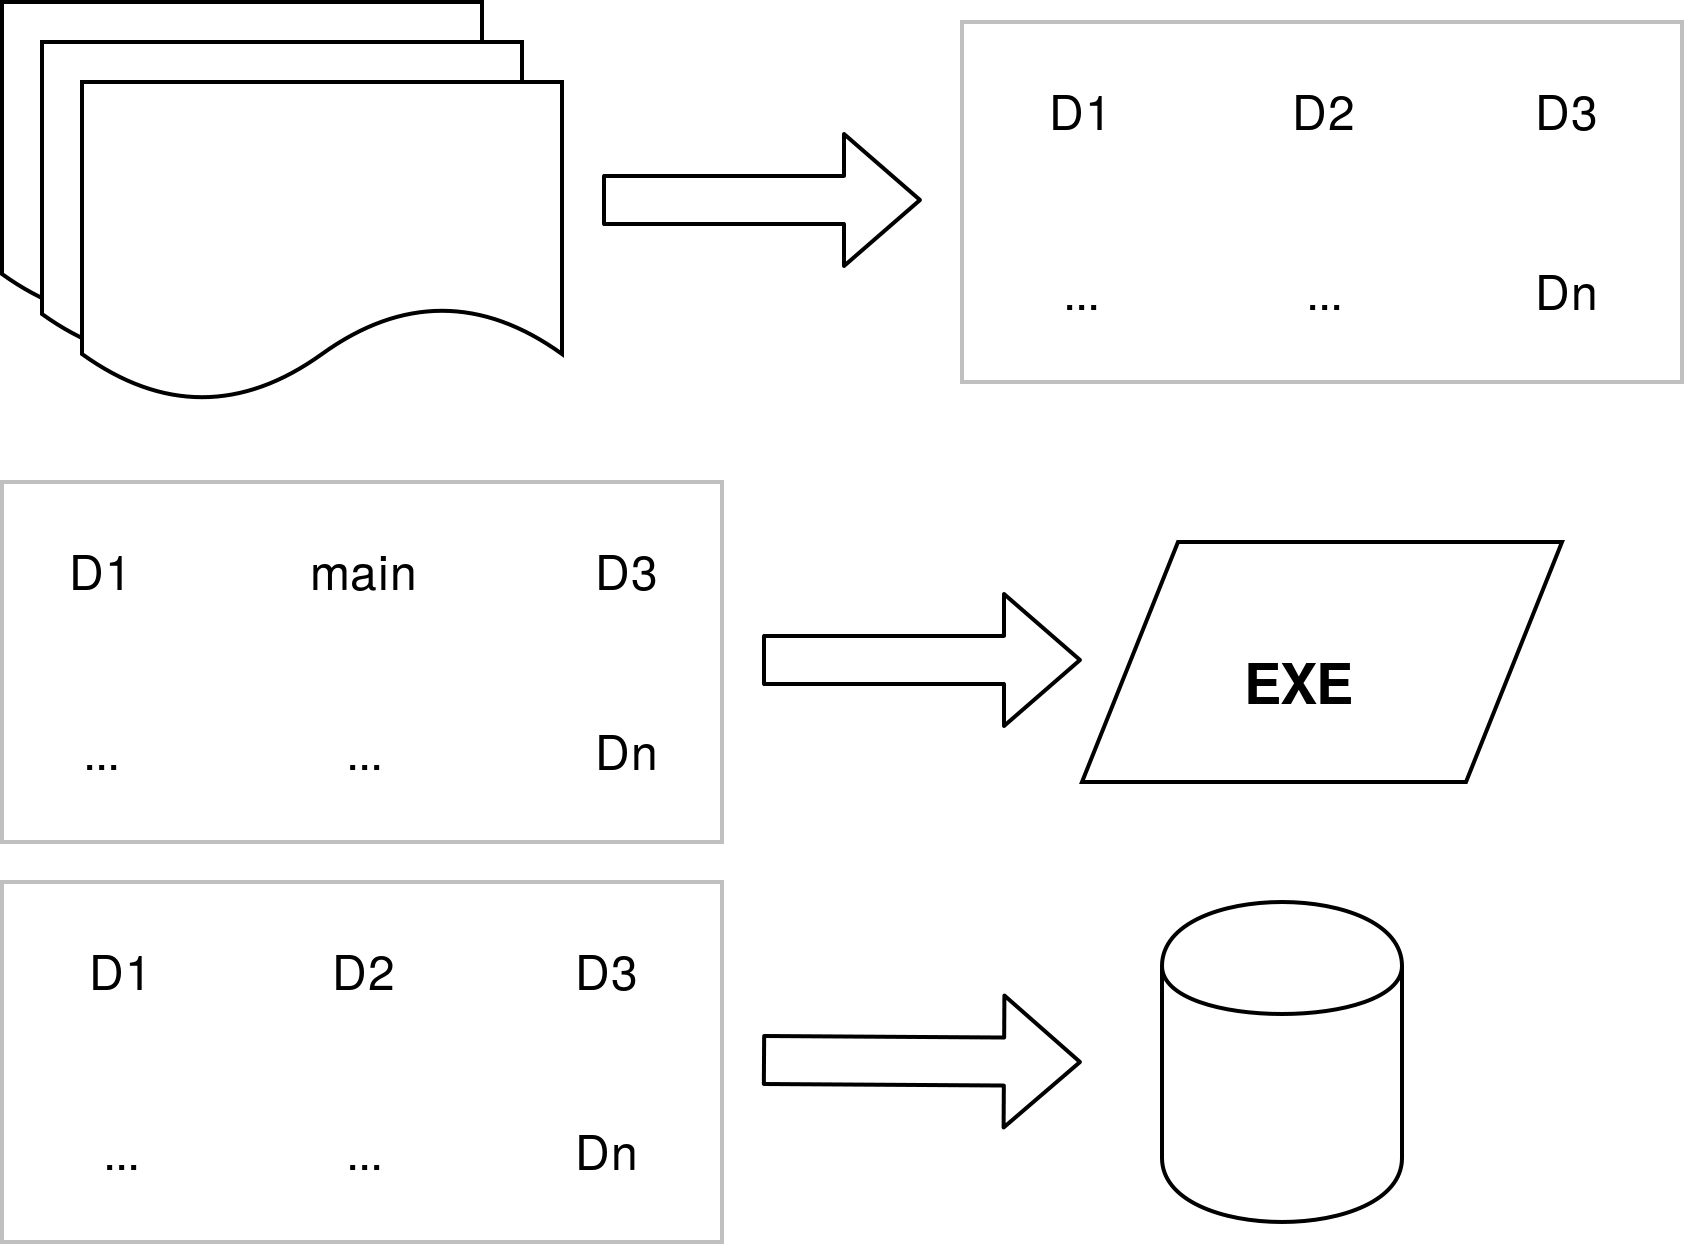
\includegraphics[align=c,width=9.5cm,keepaspectratio]{images/text_decl_bin.png}
\end{frame}

\begin{frame}[fragile]{Комментарии}
  \begin{lstlisting}
  /* Comment */

  /*
   * Multi-line comment
   */

  // Single-line comment

  //
  //
  // Fancy comment formatting
  //
  \end{lstlisting}
\end{frame}

\begin{frame}[fragile]{Основные этапы трансляции}
  \begin{enumerate}
    \item Склейка строк через \lstinline{\} \vspace{1em}
    \item Предварительная токенизация (комментарии, пробелы, базовые токены) \vspace{1em}
    \item Препроцессор ($\forall I \rightleftharpoons 1\dotso3$) \vspace{1em}
    \item Склейка смежных строковых литералов \vspace{1em}
    \item Компиляция \vspace{1em}
    \item Компоновка
  \end{enumerate}
\end{frame}

\begin{frame}[fragile]{Базовые токены}
  \begin{itemize}
    \item идентификаторы
    \item числовые токены
    \item символьные, строковые литералы и аргументы \lstinline{#include}
    \item операторы и символы пунктуации
    \item иное
  \end{itemize}
  \vspace{1em}
  \begin{lstlisting}
    a+++++b   // a ++ ++ + b
    a++ + ++b // a ++ + ++ b
    1E+12 // OK
    0x1E+12 // bad
    0x1E +12 // OK
  \end{lstlisting}
\end{frame}

%-------------------------------------------------
\section{Функция main}

\begin{frame}[fragile]{Функция main}
  \begin{itemize}
    \item нельзя явно вызвать
    \item нельзя взять адрес
    \item не может быть автоматически сгенерирована
    \item не может быть перегружена
    \item не может иметь спецификаторов \lstinline{inline}, \lstinline{static}, \lstinline{constexpr}
  \end{itemize}
  \vspace{1em}
  \begin{lstlisting}
    int main() { /* body */ }
    int main(int argc, char * argv[]) { /* body */ }
  \end{lstlisting}
  \vspace{1em}
  \begin{itemize}
    \item вызывается после инициализации глобальных переменных
    \item выход из \lstinline{main} $\equiv$ завершение программы
    \item \lstinline{return 0;} автоматически генерируется в конце тела
  \end{itemize}
\end{frame}

%-------------------------------------------------
\section{Базовые элементы программы}

\begin{frame}[fragile]{Идентификаторы}
  \begin{itemize}
    \item \lstinline{[A-Za-z_][A-Za-z0-9_]*} \vspace{1em}
    \item совпадающие с ключевыми словами -- зарезервированы \vspace{1em}
    \item содержащие \lstinline{__} -- зарезервированы \vspace{1em}
    \item начинающиеся с \lstinline{_[A-Z]} -- зарезервированы \vspace{1em}
    \item начинающиеся с \lstinline{_} -- зарезервированы в глобальном пространстве имён
  \end{itemize}
\end{frame}

\begin{frame}[fragile]{Неквалифицированные идентифицирующие выражения}
  \begin{itemize}
    \item корректно определённые идентификаторы \vspace{0.5em}
    \item имя перегруженного оператора \lstinline{operator ==} \vspace{0.5em}
    \item имя оператора пользовательского преобразования типа \lstinline{operator bool} \vspace{0.5em}
    \item имя оператора пользовательского литерала \lstinline{operator "" _km} \vspace{0.5em}
    \item имя шаблона со списком аргументов \lstinline{T<a, b, c>} \vspace{0.5em}
    \item символ \lstinline{~} с последующим именем класса \lstinline{~Foo} \vspace{0.5em}
    \item \lstinline{~decltype(x)}
  \end{itemize}
\end{frame}

\begin{frame}[fragile]{Квалифицированные идентифицирующие выражения}
  \begin{lstlisting}
    int a = 13;

    struct C
    {
      int get() const
      { return a; }

      int get2() const
      { return ::a; }

      int get3() const
      { return ::C::a; }

      static int a = 111;
    };

    int b = C::a;
  \end{lstlisting}
\end{frame}

\begin{frame}[fragile]{Имена}
  Имя -- идентифицирующее выражение, связанное с некой программной сущностью через определение. \vspace{2em}
  \begin{lstlisting}
    int a = 1; // declaration

    int f()
    {
        return a; // usage
    }
  \end{lstlisting}
  \vspace{2em}
  Использование \rarr поиск имён \rarr сущность
\end{frame}

\begin{frame}[fragile]{Литералы}
  \begin{itemize}
    \item булевские \lstinline{true}, \lstinline{false} \vspace{0.5em}
    \item целочисленные \vspace{0.5em}
    \item дробные \vspace{0.5em}
    \item символьные \lstinline{'a'} \vspace{0.5em}
    \item строковые \lstinline{"Hello\n"} \vspace{0.5em}
    \item \lstinline{nullptr}
  \end{itemize}
\end{frame}

\begin{frame}[fragile]{Целочисленные литералы}
  \begin{lstlisting}
    -1 // -(1)

    31 // decimal
    037 // octal
    0x1F // hexadecimal
    0X1f // hexadecimal
    0b11111 // binary
  \end{lstlisting}
  
  \vspace{1em}
  
  Тип десятичного литерала -- \lstinline{int}, \lstinline{long}, \lstinline{long long}. \\
  
  \vspace{1em}
  
  Типы других баз могут быть беззнаковые.
  \begin{itemize}
    \item суффикс \lstinline{u}, \lstinline{U} $\implies$ \lstinline{unsigned}
    \item суффикс \lstinline{l}, \lstinline{L} $\implies$ \lstinline{long}
    \item суффикс \lstinline{ll}, \lstinline{LL} $\implies$ \lstinline{long long}
  \end{itemize}
\end{frame}

\begin{frame}[fragile]{Дробные литералы}
  \begin{lstlisting}
    1e-5 // 10^-5
    1. // 1.0
    1.23 // 1.23
    0x1.2p-1 // 0.5625
  \end{lstlisting}
  
  \vspace{1em}
  
  Тип дробного литерала -- \lstinline{double}, либо задаётся суффиксом:
  
  \vspace{0.5em}
  \begin{itemize}
    \item \lstinline{f} \lstinline{F} $\implies$ \lstinline{float}
    \item \lstinline{l} \lstinline{L} $\implies$ \lstinline{long double}
  \end{itemize}
\end{frame}

\begin{frame}[fragile]{Операторы}
  Оператор -- элемент языка, задающий некоторое вычисление над операндами. Может иметь побочные эффекты и результат.
  
  \vspace{1em}

  \lstinline{a + b}
  
  \vspace{2em}

  Свойства:
  \begin{itemize}
    \item арность
    \item приоритет
    \item ассоциативность
  \end{itemize}
  \begin{lstlisting}
    a = b = c // a = (b = c)
    a , b, c // (a , b) , c
  \end{lstlisting}
\end{frame}

\begin{frame}{Список операторов и их свойства}
  \url{https://en.cppreference.com/w/cpp/language/operator_precedence}
\end{frame}

\begin{frame}[fragile]{Выражения}
  Операторы $+$ операнды $\implies$ выражения

  \vspace{2em}
  Первичные выражения
  \begin{itemize}
    \item литералы
    \item идентификаторы
    \item \lstinline{(} выражение \lstinline{)}
    \item лямбда-выражения
    \item выражения свёртки
  \end{itemize}

  \vspace{1.5em}
  Операнд -- первичное выражение или составное выражение.
\end{frame}

\begin{frame}{Порядок исполнения}
  Порядок исполнения выражения -- порядок вычисления подвыражений составного выражения $\implies$ не определён.
  
  \vspace{1.5em}
  
  $\succ$ <<Упорядочено до>> -- это несимметричное, транзитивное отношение между парой вычислений в рамках одного треда.
  
  \vspace{1.5em}
  
  A $\succ$ B $\implies$ A полностью завершено до B
  
  \vspace{1.5em}
  
  $\neg$ A $\succ$ B $\land$ $\neg$ B $\succ$ A $\implies$
  \begin{itemize}
    \item A и B разнесены во времени \vspace{0.5em}
    \item A и B пересекаются во времени
  \end{itemize}
\end{frame}

\begin{frame}[fragile]{Инструкции}
  \[
    P = S_1 \dotso S_n
  \]
  \begin{itemize}
    \item выражений <\emph{выражение}> \lstinline{;}
    \item блоки \lstinline|{| <\emph{инструкции}> \lstinline|}|
    \item ветвлений
    \item циклов
    \item переходов
    \item объявлений
    \item \lstinline{try} блоки
  \end{itemize}
\end{frame}

\begin{frame}{Инструкции, наглядно}
  \hspace*{3cm}
\includegraphics[align=c,width=5cm,keepaspectratio]{images/control.png}
\end{frame}

\begin{frame}[fragile]{Ветвления}
  \begin{lstlisting}
    if (err)
        std::cout << err << std::endl;

    if (x > y) {
        a = x;
    } else {
        a = y;
    }

    switch (z) {
        case 'a': return 101;
        case 'c': return 33;
        default: return -1;
    }
  \end{lstlisting}
\end{frame}

\begin{frame}[fragile]{Циклы}
  \begin{lstlisting}
    for (int i = -10; i < 10; ++i) {
        a *= i * i;
    }

    for (const auto & id : x.get_ids()) {
        std::cout << id << std::endl;
    }

    while (!q.empty()) {
        send(q.front());
        q.pop_front();
    }

    do {
        std::cout << "Hello there" << std::endl;
    } while (false);
  \end{lstlisting}
\end{frame}

\begin{frame}[fragile]{Переходы}
  \begin{itemize}
    \item \lstinline{goto} \emph{метка} \lstinline{;} \vspace{1em}
    \item \lstinline{break;} \vspace{1em}
    \item \lstinline{continue;} \vspace{1em}
    \item \lstinline{return} \emph{выражение} \lstinline{;} \vspace{1em}
    \item \lstinline{return} \emph{braced init list} \lstinline{;}
  \end{itemize}
\end{frame}

\begin{frame}[fragile]{Переменные}
  \emph{список спецификаторов} \emph{список инициализации} \lstinline{;}

  \vspace{1em}

  \emph{список спецификаторов} $\equiv$ [[\emph{спецификатор}]...] \emph{тип}

  \vspace{1em}

  \emph{список инициализаци} $\equiv$ \emph{id} [\lstinline{=} \emph{expr}] [, \emph{id} ...]

  \vspace{1em}

  \begin{lstlisting}
    int a;
    char b = '\t';
    const float x = 0.001, y = 1e+10;
  \end{lstlisting}
\end{frame}

\begin{frame}[fragile]{Область видимости}
  \begin{lstlisting}
    // no 'x' visible yet

    int x = 11;
    int main()
    {
      {
        int y = x + 2; // 13
        int x = x; // uninitialized
        x = y * 2; // 26
        {
          int z = x; // 26
        }
      }
      int z = x; // 11
      int u = y; // compilation error
    }
  \end{lstlisting}
\end{frame}

\begin{frame}[fragile]{Некоторые операторы}
  \begin{lstlisting}
    int x, y = 5; // not an assignment
    x = 1 + 2;
    y *= x / 2;
    x = ++y;
    x = y++;
    x--;
    y = -x;
    x = 10 % 4;
    x = 0b101 & 0xF;
    x = 0xC | 0xA;
    x ^= 011;
    x = 0b101 << 4;
    auto b = !x || y;
    auto bb = !x && y;
    auto bbb = x != y;
    auto bbbb = x == y;
  \end{lstlisting}
\end{frame}

\begin{frame}[fragile]{Типы}
  Объекты, выражения, функции, ... : тип

  \vspace{2em}

  \begin{itemize}
    \item базовые (фундаментальные) \vspace{1em}
    \item сложные (составные)
  \end{itemize}
  \vspace{1em}
  \begin{lstlisting}
    using T = int;

    static const int * x;
  \end{lstlisting}
\end{frame}

\begin{frame}{Базовые типы}
  \begin{itemize}
    \item \lstinline{void} \vspace{0.5em}
    \item \lstinline{std::nullptr_t} \vspace{0.5em}
    \item арифметические \vspace{0.5em}
      \begin{itemize}
        \item дробные \vspace{0.5em}
        \item интегральные \vspace{0.5em}
          \begin{itemize}
            \item логический \vspace{0.5em}
            \item символьные \lstinline{char}... \vspace{0.5em}
            \item знаковые целые \lstinline{int}... \vspace{0.5em}
            \item беззнаковые целые \lstinline{unsigned}... \vspace{0.5em}
          \end{itemize}
      \end{itemize}
  \end{itemize}
\end{frame}

\begin{frame}[fragile]{Явные и неявные приведения типов}
  \begin{lstlisting}
    float a = 10; // int -> float
    int i = -101;
    unsigned long x = 1; // int -> unsigned long
    auto y = x + i; // int -> unsigned long
    int b = 1.5; // double -> int

    int c{static_cast<int>(a)}; // explicit cast
  \end{lstlisting}
\end{frame}

\begin{frame}[fragile]{Требования к целым числовым типам}
  \scriptsize
  \centering
  \begin{tabular}{|C{8em}|C{6em}|C{6em}|S{3em}|S{3em}|S{3em}|}
    \hline
    \bfseries Тип & \bfseries Минимальное значение & \bfseries Максимальное значение & \bfseries ILP32 & \bfseries LP64 & \bfseries LLP64 \\
    \hline
    char & & & 8 & 8 & 8 \\
    signed char & -127 & 127 & 8 & 8 & 8 \\
    unsigned char & 0 & 255 & 8 & 8 & 8 \\
    \hline
    short & & & & & \\
    short int & \multirow{-2}{*}{-32767} & \multirow{-2}{*}{32767} & \multirow{-2}{*}{16} & \multirow{-2}{*}{16} & \multirow{-2}{*}{16} \\
    \hline
    unsigned short & & & & & \\
    unsigned short int & \multirow{-2}{*}{0} & \multirow{-2}{*}{65535} & \multirow{-2}{*}{16} & \multirow{-2}{*}{16} & \multirow{-2}{*}{16} \\
    \hline
    int & -32767 & 32767 & 32 & 32 & 32 \\
    \hline
    unsigned & & & & & \\
    unsigned int & \multirow{-2}{*}{0} & \multirow{-2}{*}{65535} & \multirow{-2}{*}{32} & \multirow{-2}{*}{32} & \multirow{-2}{*}{32} \\
    \hline
    long & & & & & \\
    long int & \multirow{-2}{*}{-2147483647} & \multirow{-2}{*}{2147483647} & \multirow{-2}{*}{32} & \multirow{-2}{*}{64} & \multirow{-2}{*}{32} \\
    \hline
    unsigned long & & & & & \\
    unsigned long int & \multirow{-2}{*}{0} & \multirow{-2}{*}{4294967295} & \multirow{-2}{*}{32} & \multirow{-2}{*}{64} & \multirow{-2}{*}{32} \\
    \hline
    long long & & & & & \\
    long long int & \multirow{-2}{*}{$-2^{63}-1$} & \multirow{-2}{*}{$2^{63}-1$} & \multirow{-2}{*}{64} & \multirow{-2}{*}{64} & \multirow{-2}{*}{64} \\
    \hline
    unsigned long long & & & & & \\
    unsigned long long int & \multirow{-2}{*}{0} & \multirow{-2}{*}{$2^{64}-1$} & \multirow{-2}{*}{64} & \multirow{-2}{*}{64} & \multirow{-2}{*}{64} \\
    \hline
  \end{tabular}
\end{frame}

\begin{frame}[fragile]{Требования к дробным числовым типам}
  \centering
  \begin{tabular}{|C{8em}|C{8em}|C{8em}|}
    \hline
    \bfseries Тип & \bfseries Минимальное число точно представимых десятичных цифр & \bfseries Максимально представимое число \\
    \hline
    float & 6 & 1E+37 \\
    double & 10 & 1E+37 \\
    long double & 10 & 1E+37 \\
    \hline
  \end{tabular}
\end{frame}

\end{document}
